\chapter{Background}
\section{Existing alternatives}
As of writing this paper, only very few tools support monitoring of STP topologies.
The ones we found are LoriotPro\cite{LoriotPro}, LiveAction\cite{LiveAction} and L2Discover\cite{L2Discover}.
Only the source code for L2Discover is openly available, the other two are proprietary software.
The company SolarWinds has an open vote on their website on whether or not to include this feature in the future since 2014\cite{thwackSW}.
LoriotPro and L2Discover use the SNMP for their topology discovery.
STP is only used to discover unused and duplicate links.
The Generator described in this paper uses only STP, thus not needing SNMP capable devices.

\section{Technologies used}
\subsection{STP}
\subsubsection{Port States}
The most important part of the STP is the way ports act and react.
Depending on the topology and respective configuration of the Bridges, ports can be in one of the following three states:
\begin{itemize}
    \item \textbf{Root}: The port leading to the root of the tree.
    \item \textbf{Dedicated}: Dedicated Ports are ports where packets are sent.
    \item \textbf{Blocking}: No packets are sent via a Blocking Port.
        If no superior STP packets are received on a Blocking Port for a set amount of time it transitions to Dedicated State.
\end{itemize}
%TODO: add graphic explaining port states
\subsubsection{STP Packets}
\label{stp_packet}
\begin{figure}[h]
    \centering
    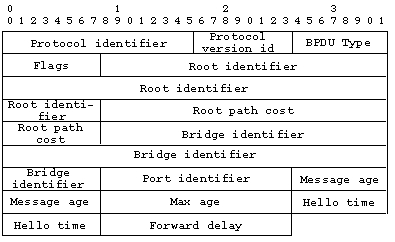
\includegraphics[width=0.8\textwidth]{stp_bpdu.png}
    \caption{An STP BPDU}
    \label{fig:stp_bpdu}
\end{figure}
In this section we will explain the parts of an STP Bridge Protocol Data Unit (BPDU), as seen in Figure~\ref{fig:stp_bpdu}, used in this project.
\begin{itemize}
    \item \textbf{Flags}: The Flags Byte is used for the \textit{Topology Change} and \textit{Topology Change Acknowledgement} flags.
    \item \textbf{Root/Bridge Identifier}: The Identifier conists of three parts and has the same layout for the Root and regular bridges:
        \begin{itemize}
            \item Priority (4 Bits): A value between 0 and 61440 configurable in increments of 4096
            \item System ID Extension (12 Bits): Used for keeping the Bridge ID unique if multiple VLANs are configured for a Bridge
            \item Bridge MAC (6 Byte): The MAC address of the Bridge
        \end{itemize}
        The conjunction of these three parts is used in comparisons as one large 8 Byte number.
    \item \textbf{Root Path Cost}: The Root Path Cost is the sum of all Port Costs (which can be configured in the Bridge) along the current path. The Root Path Cost in packets sent by the Root is 0.
    \item \textbf{Message Age}: The Message Age is the number of Bridges that have been passed (in addition to the Root) along the current path.
    \item \textbf{Forward Delay}: After this time, if no superior packet was received, a Root, or Blocking Port will transition to Dedicated.
        Note that if a Root Port transitions to Dedicated state that means the Bridge now assumes it is the Root.
\end{itemize}
\subsubsection{Spanning Tree Algorithm}
STP enabled Bridges run through the following algorithm on a received packet:
How does STP work?
\begin{algorithm}
    \DontPrintSemicolon
    \KwData{\\
    $received$ = received packet\;
    $current$ = data of the current Bridge\;
    }
    \;
    \If{$received.rootId < current.rootId$}{
        \tcc{There is a new Root in the network}
        $current.rootId=other.rootId$\;
        set receiving port as Root-Port\;
        set other ports to Dedicated\;
    }{
        \uIf{$received.rootPathCost<current.rootPathCost$}{
            \tcc{This means that the path via the other Bridge is shorter, so this should be our new Root-Path}
            set receiving port as Root-Port\;
            set other ports to Dedicated\;
        }
        \ElseIf{$received.rootPathCost==current.rootPathCost \land received.bridgeId<current.bridgeId$}{
            \tcc{Both Bridges are equidistant from the Root, but the other Bridge has a lower Bridge Identifier and should be the Dedicated Bridge on the connection}
            set receiving port as Blocking Port\;
        }
        \tcc{Finally check if the transitions described in section \ref{stp_packet} on \textbf{STP Packets} is necessary}
        doPacketTimeOutTransitions()\;
    }
    
    \caption{Spanning Tree Bridge Algorithm}
\end{algorithm}
\subsection{PCAP}
PCAP 
\subsection{JSON}
JSON very brief
